\chapter{Z Tanım Bölgesinde Zaman Tanım Bölgesi İsterler}
Zaman tanım bölgesi isterleri s tanım bölgesinde tanımlanmıştır ve z tanım bölgesine 
\begin{equation}
    z=e^{sT}
\end{equation}
ile geçiş yapılmaktadır. Bu durumda s tanım bölgesinde isterlerin karşılık düştüğü konumlar bir dönüşüm sonucu z tanım bölgesinde konumlanmaktadır. S tanım bölgesinde bir kutup
\begin{equation}
    s=-\sigma+w_di
\end{equation}
olmak üzere z tanım bölgesinde
\begin{equation}
\begin{split}
    z&=e^{-\sigma T+w_dTi}\\
    z&=e^{-\sigma T}e^{w_dTi}\\
    z&=e^{-\sigma T}\phase{w_dT}\\
    z&=e^{-\sigma T}\cos{w_dT}+e^{-\sigma T}\sin{w_dT}i\\
    z&=e^{-\zeta w_n T}\cos{(\sqrt{1-\zeta^2}w_nT)}+e^{-\zeta w_n T}\sin{(\sqrt{1-\zeta^2}w_nT)}i
\end{split}
\end{equation}
olarak elde edilir. Görüldüğü üzere s tanım bölgesinden z tanım bölgesine geçiş durumunda kutupsal koordinatlar elde edilmektedir. İncelemelerin basit olması amacıyla örnekleme zamanı $T=1$ olsun.
$w_n=1$ olmak üzere
\begin{equation}
        z=e^{-\zeta}\phase{\sqrt{1-\zeta^2}}
\end{equation}
elde edilir. $\zeta$ arttıkça yarıçap küçülmektedir ve açı azalmaktadır. Çizelge~\ref{tbl:yaricap_aci1} ile verilene göre yarıçapın küçüldüğü ve açının azaldığı görülmektedir.
\begin{table}[!htb]
    \centering
    \caption{$w_n=1$ için yarıçap ve açının değişimi}\label{tbl:yaricap_aci1}
    \begin{tabular}{cc}\hline
        Yarıçap& Açı\\\hline
        $0.9048$& $57.0086^o$\\
        $0.8187$& $56.1382^o$\\
        $0.7408$& $54.6567^o$\\
        $0.6703$& $52.5124^o$\\
        $0.6065$& $49.6196^o$\\
        $0.5488$& $45.8366^o$\\
        $0.4966$& $40.9174^o$\\
        $0.4493$& $34.3775^o$\\
        $0.4066$& $24.9747^o$\\
        $0.3679$& $0^o$\\\hline
    \end{tabular}
\end{table}

\begin{figure}[!htb]
    \centering
    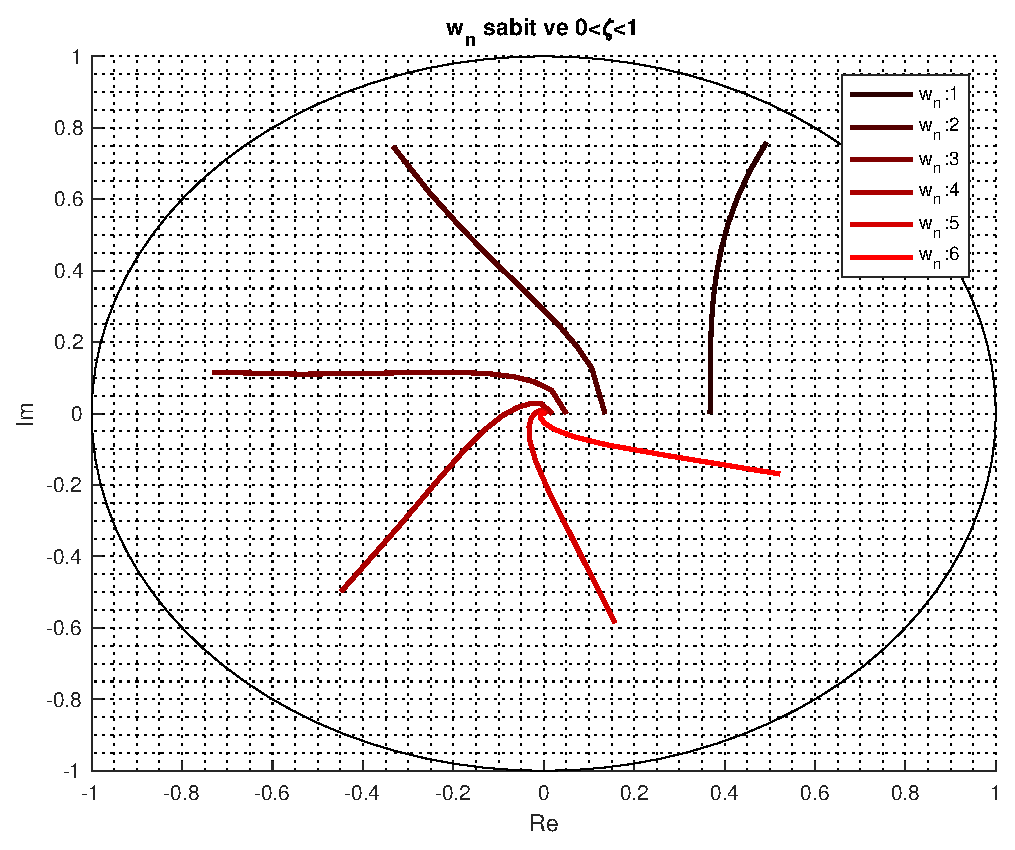
\includegraphics[width=0.75\textwidth]{img/lec6_plot1}
    \caption{$\zeta$ değişiminin z tanım bölgesindeki izdüşümü}
    \label{fig:lec6_plot1}
\end{figure}
%%%%%%%%%%%%%%%%%%%%
$\zeta=0.1$ olmak üzere
\begin{equation}
        z=e^{-0.1w_n}\phase{0.995w_n}
\end{equation}
elde edilir. $w_n$ arttıkça yarıçap küçülür ve açı artar. 
\begin{table}[!htb]
    \centering
    \caption{$\zeta=0.1$ için yarıçap ve açının değişimi}\label{tbl:yaricap_aci2}
    \begin{tabular}{cc}\hline
        Yarıçap& Açı\\\hline
        $0.90484$&  $57.009^o$\\
        $0.81873$&  $114.02^o$\\
        $0.74082$&  $171.03^o$\\
        $0.67032$&  $228.03^o$\\
        $0.60653$&  $285.04^o$\\
        $0.54881$&  $342.05^o$\\\hline
    \end{tabular}
\end{table}

\begin{figure}[!htb]
    \centering
    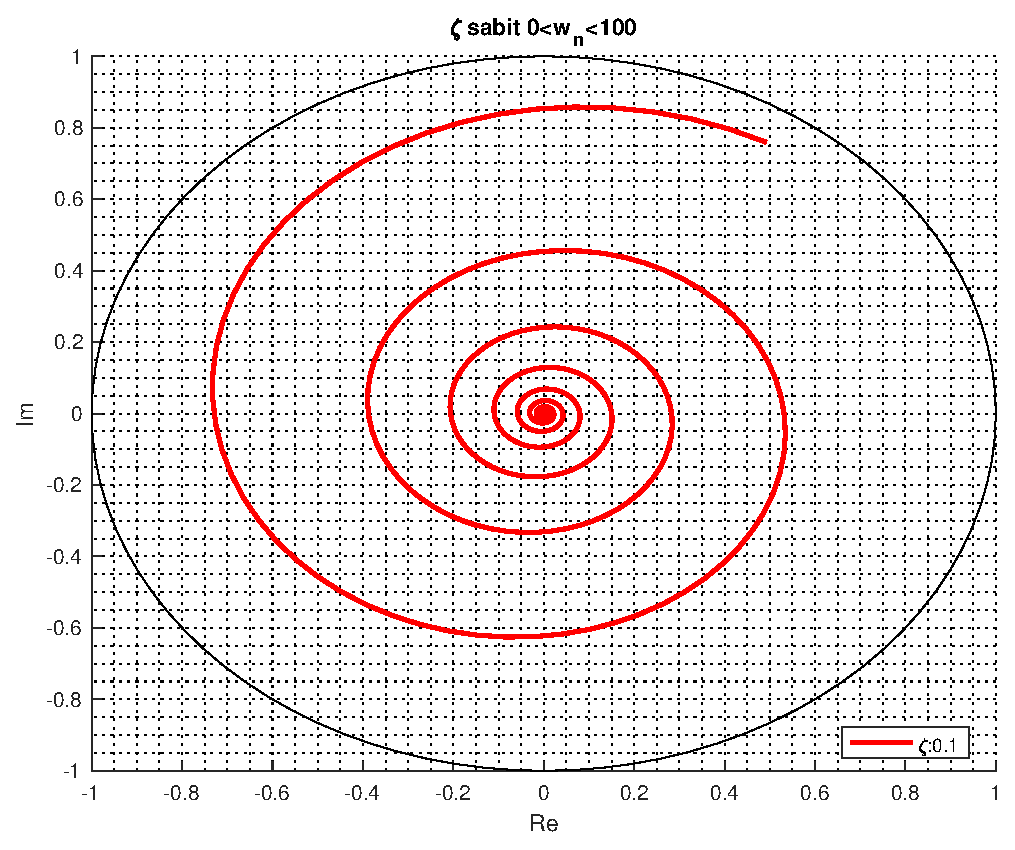
\includegraphics[width=0.75\textwidth]{img/lec6_plot2}
    \caption{$w_n$ değişiminin z tanım bölgesindeki izdüşümü($\zeta=0.1$)}
    \label{fig:lec6_plot2}
\end{figure}

\begin{figure}[!htb]
    \centering
    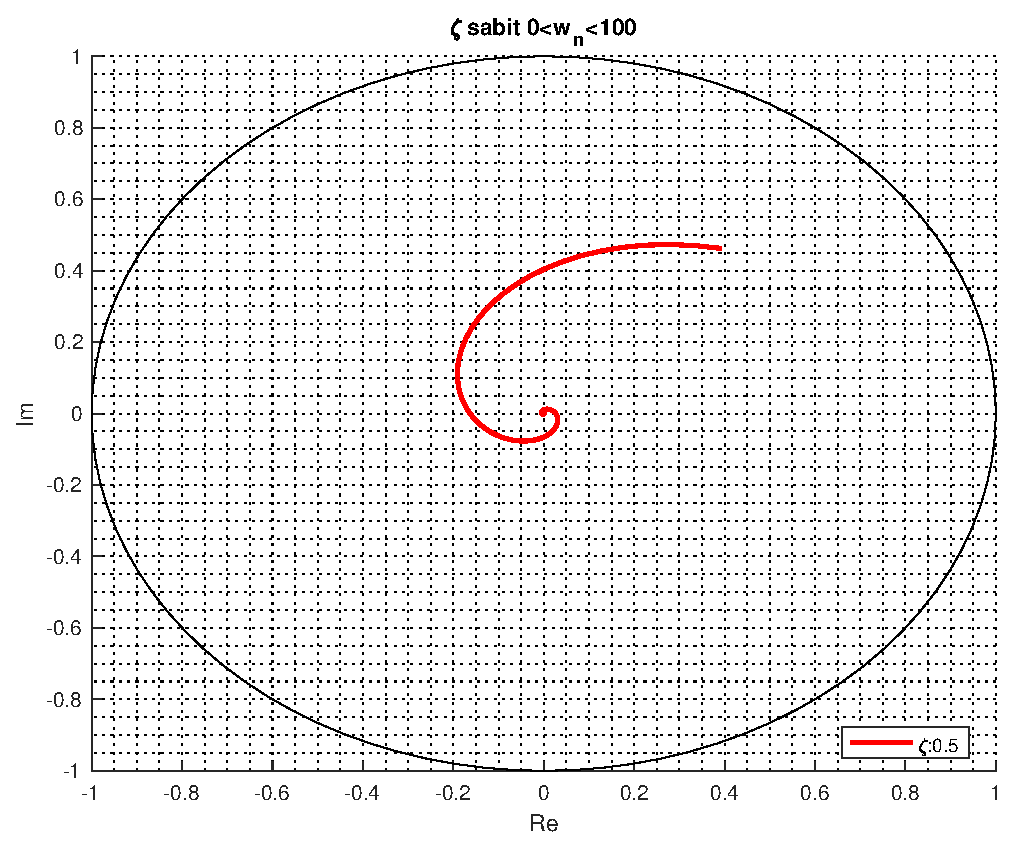
\includegraphics[width=0.75\textwidth]{img/lec6_plot3}
    \caption{$w_n$ değişiminin z tanım bölgesindeki izdüşümü($\zeta=0.5$)}
    \label{fig:lec6_plot3}
\end{figure}
%%%%%%%%%%%%%%%%%%%%
$t_s=5$ ise $\zeta w_n=0.8$ olur ve 
\begin{equation}
\begin{split}
    z&=e^{-\zeta w_n}\phase{\sqrt{1-\zeta^2}w_n}\\
    z&=e^{-0.8}\phase{\sqrt{1-\zeta^2}\frac{0.8}{\zeta}}
\end{split}
\end{equation}
elde edilir. $\zeta$ arttıkça yarıçap değişmez ve açı azalır. 
\begin{table}[!htb]
    \centering
    \caption{$t_s=5$ için yarıçap ve açının değişimi}\label{tbl:yaricap_aci3}
    \begin{tabular}{cc}\hline
        Yarıçap& Açı\\\hline
        $0.44933$& $224.55^o$\\
        $0.44933$& $105.02^o$\\
        $0.44933$& $61.115^o$\\
        $0.44933$& $34.377^o$\\
        $0.44933$& $     0^o$\\\hline
    \end{tabular}
\end{table}

\begin{figure}[!htb]
    \centering
    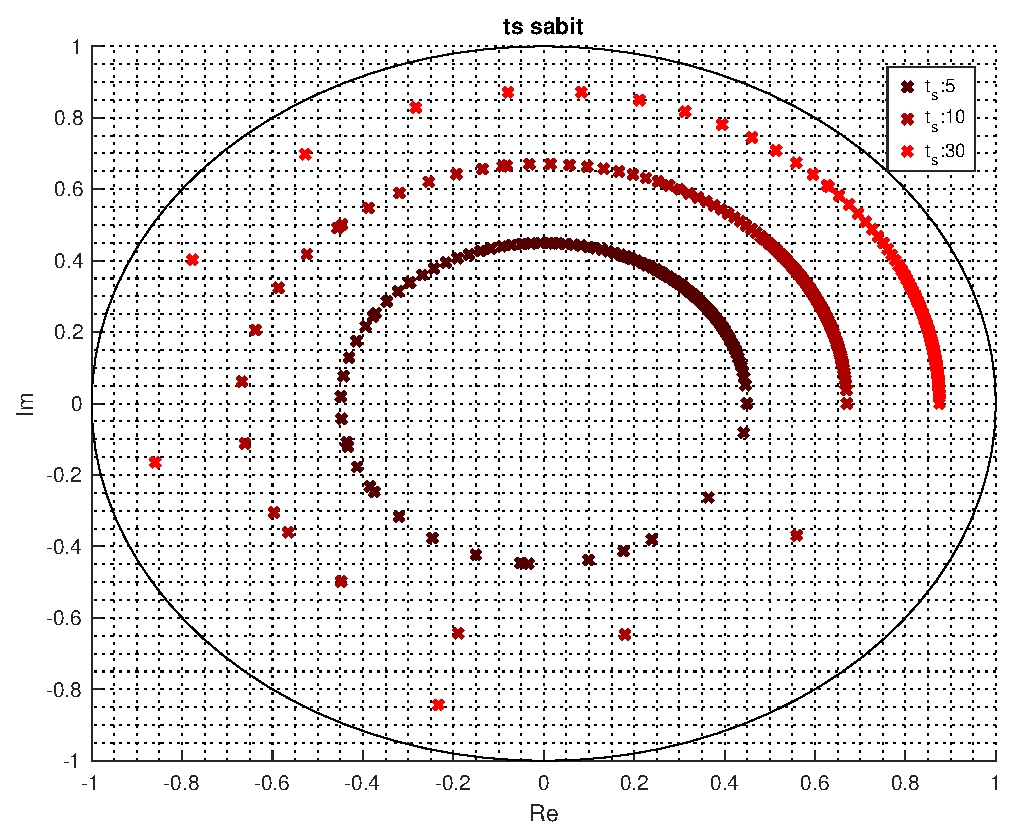
\includegraphics[width=0.75\textwidth]{img/lec6_plot4}
    \caption{$t_s$ sabit durumunun z tanım bölgesindeki izdüşümü}
    \label{fig:lec6_plot4}
\end{figure}

